\section{Aanpak}
\label{Aanpak}
Een van de eerste beslissingen die genomen moest worden heeft betrekking op de architectuur van het systeem. 
Al snel bleek dat de opdrachtgever een voorkeur had voor een webapplicatie die door het hele Erasmus MC op het netwerk simpel en snel gebruikt kon worden. 
Voor onze Image Processing kregen wij het advies van Dr. Botha om een aantal Python bibliotheken te bekijken en deze indien mogelijk te gebruiken. 
\\
\\
De combinatie van deze feiten leidde ons richting Django, wat een Python framework is voor het bouwen van websites met Python. 
Na wat onderzoek en naar aanleiding van de ervaringen die \'{e}\'{e}n van de projectleden al had met Django hebben we ervoor gekozen om Django te gaan gebruiken. 
\\
\\
Voor wat betreft de visuele interactie hebben we gekeken naar verschillende JavaScript bibliotheken. Mede door de uitgebreide ervaringen van diverse leden hebben we uiteindelijk gekozen voor de combinatie van Prototype en Scriptaculous.
\\
\\
Tijdens het project bleek uiteindelijk dat er behoefte was aan een tekenapplicatie binnen de omgeving. Deze was niet te realiseren via JavaScript en dus is er uiteindelijk ook nog een Flash-applicatie geschreven die communiceert met JavaScript.

\subsection{Project gerelateerd}
\label{aanpak_project_gerelateerd}
In de beginperiode hebben wij ons ingelezen op de basis anatomische kennis die nodig was om de experts van het Erasmus MC te kunnen volgen.
Hierbij hebben we vooral veel gebruik gemaakt van de kennis van \'{e}\'{e}n van de groepsleden, die voor ze aan deze studie begon drie jaar werkzaam was als radiodiagnostisch laborant. Ook zijn we een dag langs geweest bij het Erasmus MC en hebben daar een rondleiding gehad door het laboratorium en de snijzalen waar onderzoek wordt gedaan. 
\\
\\
Een andere uitdaging was de relatief grote groep studenten voor dit project. 
Om te voorkomen dat we elkaar te veel in de weg zouden zitten hebben we de diverse delen van het project opgesplitst en de taken duidelijk verdeeld. 
Daarnaast hebben we gebruik gemaakt van software zoals Trac, dit is een Project Management Systeem. 
Er was een locatie op de TU Delft geregeld waar we iedere dag hebben gewerkt en waar we elke ochtend een werkoverleg over wat er die dag zou moeten gebeuren konden hebben. 
Hierdoor bleef iedereen goed op de hoogte van de status van het gehele project.

\subsection{Database systeem}
\label{aanpak_database_systeem}
Het database systeem is het onderdeel van het project dat dient om de gebruikte foto's overzichtelijk in te delen in verschillende projecten. Hiervandaan wordt de gebruiker in staat gesteld om de handelingen te verrichten die nodig zijn om analyse te plegen op foto's. Typische handelingen zijn bijvoorbeeld: 

\begin{itemize}
\item Aangeven van herkenningspunten bij de foto's
\item Afbeeldingen tekenen over foto's om belangrijke gebieden aan te geven, ook wel bitmaps genoemd
\item Verschillende doorzichtige foto's over elkaar heen leggen om de verschillen te bekijken
\item Toevoegen van relevante papers en websites bij een project
\item Tags toevoegen bij projecten om ze te categoriseren
\item Vastleggen van interessante configuraties om de foto's en bijbehorende informatie te tonen, ook wel states genoemd
\item Afstanden meten in foto's
\item Een knop aanbieden om een Point Distribution Model te cre\"{e}ren
\end{itemize}

\noindent Zoals in de paragraaf Aanpak al aangegeven, zouden we gaan werken met Django en moest het product beschikbaar worden als webapplicatie.
Django is een Model View Controller opgebouwde taal.
Dat wil zeggen dat het datamodel en de functionaliteit met betrekking tot het datamodel gescheiden zijn van de gebruikersinterface en de functionaliteit met betrekking tot de gebruikersinterface.
Django heeft ook een duidelijke abstractielaag voor het database gedeelte, een Object-Relational Database Mapping.
Deze maakt het mogelijk om in een object\-ge\"{o}rienteerde taal te programmeren, maar de aangemaakte objecten worden direct gemapt op een relationele structuur. Hierdoor kunnen de objecten kunnen worden opgeslagen in een relationele database, dit verlicht de implementatie aanzienlijk.
Na diverse brainstorm sessies zijn we uiteindelijk uitgekomen op een klasse-diagram (Figuur \ref{fig:databasediagram}) dat de basis zou gaan vormen voor het database systeem.
\\
\\
\begin{figure}[htbp]
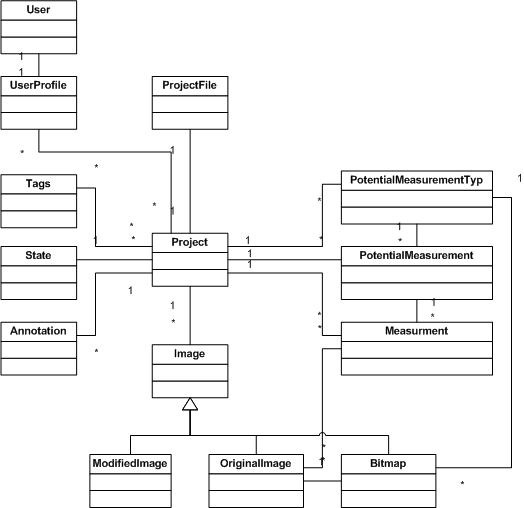
\includegraphics[width=\textwidth]{databasediagram}
\caption{Klassediagram van de database}
\label{fig:databasediagram}
\end{figure}
\\
\\
Ook het gebruikers\-beheer is standaard een onderdeel van Django, waardoor dit voor een groot deel niet meer door ons gedaan zou hoeven worden.
\\
\\
Voor de interface hebben we ervoor gekozen om veel gebruik te maken van JavaScript en zijn bibliotheken. Dit gaf ons eenvoudige toegang tot diverse visuele effecten, zoals drag en drop, fade en de sliders. Daarnaast konden we met behulp van JavaScript gebruik maken van de AJaX techniek, hiermee konden we server verzoeken sturen en de pagina updaten zonder dat de gebruiker hier last van had.
\\
\\
In de ontwerpfase is besloten dat het mogelijk moet zijn om datasets tussen gebruikers uit te wisselen. Om te zorgen dat gebruikers verschillende projecten kunnen uitwisselen is hier al in een vroeg stadium rekening mee gehouden. Er is voor gekozen alle objecten die worden gebruikt op te slaan met Universal Unique ID's, dat wil zeggen dat de kans dat bij het kopi"{e}ren van objecten objecten een zelfde identificator hebben zodanig klein is, dat hij wordt beschouwd als niet bestaand. Hierdoor is het mogelijk om datasets tussen verschillende databases uit te wisselen zonder dat er conflicten optreden.

\subsection{Image Processing}
\label{aanpak_image_processing}
De doelen op Image Processing gebied waren: het in kaart brengen van de variaties per landmark en het morphen van getekende structuren (bijvoorbeeld zenuwen of venen) naar een standaardview. Zo kunnen structuren die van verschillende foto's afkomen toch op \'{e}\'{e}n foto worden afgebeeld.

\subsubsection{Point Distribution Model}
Om het eerste doel te bereiken hebben we gebruik gemaakt van een subonderdeel van een volledig Active Shape Model, namelijk het Point Distribution Model. Het Active Shape Model is ontwikkeld door Tim Cootes. In de paper \emph{'An Introduction to Active Shape Models'} licht hij de theorie toe.\cite{introASM}
\\
\\
Waar het Active Shape Model zich bezighoudt met het automatisch herkennen van structuren binnen een foto, is het Point Distribution Model \cite{pdm} in staat om gegeven een aantal landmarks (van hetzelfde type) op verschillende foto's het gemiddelde en de hoofdassen van variatie weer te geven. Een landmark is een punt dat zo is gekozen dat het in iedere foto te vinden is en duidelijk op iedere foto te vinden is. De landmarks die gebruikt worden voor het Point Distribution Model moeten informatie geven over het verloop van een structuur, bijvoorbeeld het aangeven van het verloop van een bepaalde vene.

\subsubsection{Thin Plate Spline Transformatie}
Om het tweede doel te bereiken, het morphen van getekende structuren, is er gebruik gemaakt van een Thin Plate Spline Transformatie (TPS). Om de TPS transformatie uit te voeren zijn landmarks nodig die bepalend zijn voor de vorm van een object. Hierbij kan gedacht worden aan een set van landmarks die bestaat uit bony landmarks\footnote{landmarks die voortkomen uit de anatomie van het menselijk lichaam en voelbaar zijn vanaf de buitenkant}, landmarks die de grenzen van het object aangeven en landmarks die zich op gelijke afstanden van voorgaande landmarks bevinden. 
Impliciet zit er in dit doel nog een Image Processing doel verwerkt, namelijk het aangeven van lijnen, gebieden of punten die interessant zijn voor de onderzoeker. We hebben ervoor gekozen om de onderzoeker dit realtime in de applicatie te laten doen door het gebruik van Flash.


\subsubsection{Tekenen}
Impliciet zit er in het tweede doel nog een Image Processing doel verwerkt, namelijk het aangeven van lijnen of gebieden die interessant zijn voor de onderzoeker. We hebben ervoor gekozen om de onderzoeker dit in de browser te laten doen als ge\"{i}ntegreerd tekenprogramma. Hierbij zal het mogelijk zijn elke foto als achtergrond te kiezen en hieroverheen met \'{e}\'{e}n kleur bepaalde gebieden aan te geven.
\\
\\
Binnen de browsers zou dit tekenprogramma gemaakt kunnen worden door gebruik te maken van Canvas, een onderdeel van de nieuwe HTML-standaard, maar deze wordt nog niet ondersteund door Internet Explorer 6. Omdat we tijdens de keuze van de techniek er vanuit gingen dat het systeem in Internet Explorer 6 moest draaien, hebben we gekozen om niet Canvas maar Flash te gebruiken. Dit vereist een plugin in de browser, die op vrijwel elk systeem al aanwezig is.
\\
\\
Over de theoretische achtergrond van de verschillende gebruikte technieken is meer te vinden in het ori\"{e}ntatieverslag.
